\documentclass[11pt]{article}
\usepackage{paralist}
\usepackage{geometry}
\geometry{letterpaper}
\usepackage{graphicx}
\usepackage{amssymb}
\usepackage{amsmath}
\usepackage{bbm}
\usepackage{enumerate}
\usepackage{multirow}
\usepackage{hyperref}

\title{HMM}
\author{}
\date{}

\begin{document}
\maketitle

%%Introduction%%
Since the MILK command language tends to be much more verbose than the recipes themselves, it is essential for us to allow multiple, related MILK commands to map into a single sentence. In order to do so, we developed a HMM-like model to segment the sequential commands into coherent sentence groups. In our model, the hidden variables, $y_1,\dots,y_n$ can take on values $1,2,\dots,k$ representing the number of MILK commands that generate a single sentence. The visible variables $x_1,\dots,x_n$ are sequences of commands up to length $k$. To simplify matters and avoid sparsity issues, we simply concern ourselves with the MILK commands, disregarding their parameters. Furthermore we ignore all $\emph{create\_ing}$ and $\emph{create\_tool}$ commands, since each of those commands forms a sentence. In the vast majority of cases, no more than 4 MILK commands correspond to a single sentence. To generate English, we first tackled the problem of segmenting the sequential MILK command into coherent groups, so that multiple, related MILK commands may generate a single sentence. An illustration of our model can be seen in Figure \ref{hmm_gm} below.\\

\begin{figure}[h!]
\begin{center}
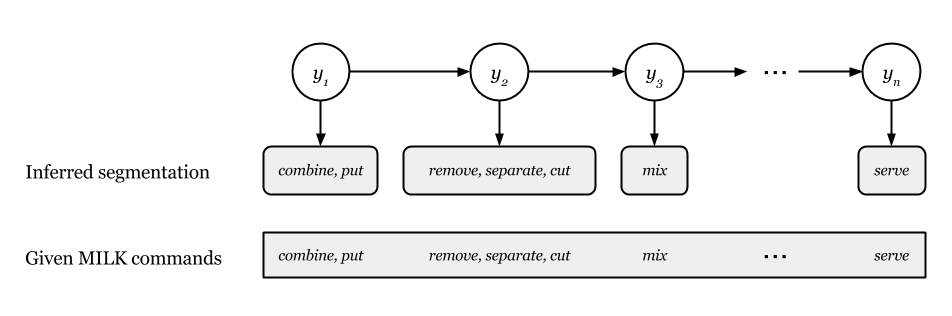
\includegraphics[width=1\textwidth]{hmm_graphical_model}
\end{center}
\caption{Graphical model for the HMM-variant}
\label{hmm_gm}
\end{figure}

%%Dataset preprocessing%%
%Our training data consists of a set of recipes. Each recipe is a sequence of English sentences with their corresponding MILK commands. In this part, we only keep the MILK predicate for each MILK command. So each recipe becomes a sequence of English sentences with MILK predicates. We also remove those commands of which the predicates are \emph{Create\_ing} and \emph{Create\_tool}, since we can safely (really?) move those commands in front of all the others for a recipe, each of those commands becomes one group.\\

%HMM in detail
% A HMM is a generative model that generates both the label sequence and the observation sequence. The label sequence is generated from a Markov model at first, then the observation sequence is generated from the label sequence.

In our hidden Markov model, the MILK commands segmentation reduces to a sequence labeling problem. The input is a sequence of MILK commands of length $n$: $x_1,\dots, x_n$. The output is another sequence $y_1, \dots, y_n$ representing the generated sentence groups. During training time, we estimate the HMM parameters $\sigma$ and $\tau$ by maximum likelihood estimation based on our preprocessed training recipes, each of which is a sequence of MILK commands with their group labels:

%% formula of sigma and tau %%
$$\hat{\sigma}_{y,y'} = \frac{n_{y,y'}(\textbf{y})}{n_{y,o}(\textbf{y})}, \,\,\,\,\,\,\,\,\,\,\,\,\,\,\,
\hat{\tau}_{y,x} = \frac{n_{y,x}(\textbf{x,y})}{n_{y,o}(\textbf{x,y})}$$
where, $n_{y,y'}$ is the number of times label $y'$ followed by $y$ and $n_{y,x}$ is the number of times $x$ is labeled as $y$. To deal with the sparse data problem, we compute the smoothed $\tilde{\tau}_{y,x}$ by adding a pseudo-count $\alpha$:
%% formula of smoothed tau %%
$$\tilde{\tau}_{y,x} = \frac{n_{y,x}(\textbf{x,y})+\alpha}{n_{y,o}(\textbf{x,y})+\alpha|W|}$$
where $|W|$ represents the total count of MILK commands in the training data. We perform a line search based on our held-out data to choose the best $\alpha$ among a set of candidate values.\\

During testing time, given the estimated $\hat{\sigma}$, $\tilde{\tau}$ parameters and a sequence of MILK commands, we perform the Viterbi algorithm to find the most likely label sequence $\textbf{y}$. In fact, we adapt the algorithm to find the top-$k$ most likely sequences of labels.
%Given a posterior $y$, it corresponds exactly to a segmentation of the MILK commands
% At last, we create the MILK command segmentation based on the labels.
Finally, we recover the MILK command segmentation based on the labels.
\\

To evaluate our model, we compared the Viterbi segmentations to the true ones by treating every boundary between MILK commands as an individual binary classification problem. Finally, we considered the F-score of our model combined over all sentences in our test set. Our average F-score was on average 0.766 for $\alpha=10^{-5}$.\\

%Just-in-time HMM
This is the first part in our MILK-to-English pipeline. The segmentation result is to be used in a ``just-in-time'' way: As we go through a sequence of MILK commands, at command $x_i$, we wish to know the distribution over the number of commands that follow $x_i$ and should be grouped together with $x_i$ to form a sentence. We compute these distributions by simply counting the corresponding frequencies in our $k$ best sequences.

% - what is the probability distribution of all possible groupings.
% We compute the counting frequencies of $y_i$ using our $k$ best sequences to create the probability distribution. With the probabilities provided, we choose a grouping number and go next.

\end{document}
